% MH1812 — Chapter 5: Counting (0->100 ground-up)
\chapter[Counting]{Counting: Product, Sum, Permutations, Combinations and Pigeonhole}
\label{ch:counting}

\begin{quote}
\emph{``Counting is the oldest intellectual art.''} Algorithms enumerate possibilities; combinatorics tells us how many there are --- without listing them all.
\end{quote}

\noindent\fbox{\parbox{\dimexpr\linewidth-2\fboxsep-2\fboxrule}{%
\textbf{From zero: choices as branches.} Picture decisions as a tree: each level = a choice, each leaf = an outcome. We derive product/sum rules from tree width, then count orderings (permutations) and selections (combinations), and finally the pigeonhole principle that forces collisions.}}
\vspace{0.4em}

\section*{Learning Outcomes}
After this chapter you will be able to:
\begin{enumerate}[label=(L\arabic*)]
    \item apply product and sum rules to sequential and alternative choices;
    \item count permutations $P(n,r)$ and combinations $\binom{n}{r}$ and relate them;
    \item use complement and inclusion--exclusion to simplify counting;
    \item apply the pigeonhole principle and its generalised form;
    \item solve stars-and-bars and distribution problems.
\end{enumerate}

% ============================================================
\section{Product and Sum Rules}
\label{sec:product-sum}
\begin{definition}[Product rule]
If a procedure breaks into $k$ sequential stages with $n_i$ choices at stage $i$ (independent of earlier choices), total outcomes $=n_1n_2\cdots n_k$.
\end{definition}
Picture: a $k$-level tree where each node at level $i-1$ sprouts $n_i$ children --- leaves $=\prod n_i$.

\begin{definition}[Sum rule]
If tasks $T_1,\dots,T_k$ are disjoint (no overlap), with $n_i$ ways for $T_i$, total ways for ``do some $T_i$'' $=\sum n_i$.
\end{definition}

\begin{figure}[h]\centering
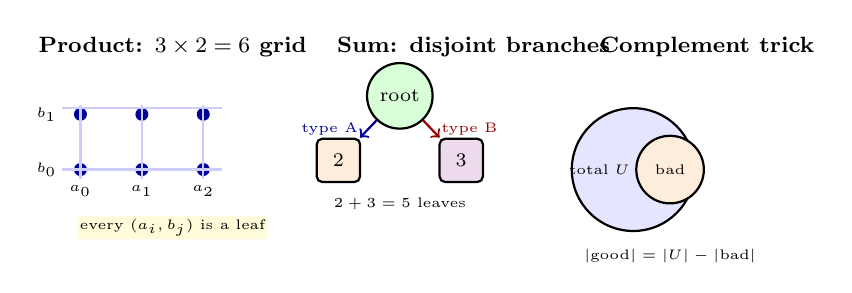
\begin{tikzpicture}[scale=0.78,every node/.style={font=\scriptsize}]
% Product rule grid and sum rule branches
\begin{scope}
\node[font=\footnotesize\bfseries] at (1.5,2.0) {Product: $3\times2=6$ grid};
\foreach \x in {0,1,2} \foreach \y in {0,1} \fill[blue!60!black] (\x*1.0,\y*0.9) circle (3pt);
\foreach \x in {0,1,2} \node[font=\tiny] at (\x*1.0,-0.35) {$a_{\x}$};
\foreach \y in {0,1} \node[font=\tiny] at (-0.55,\y*0.9) {$b_{\y}$};
\draw[thick,blue!20] ( -0.3,-0.15) grid (2.3,1.05);
\node[font=\tiny,fill=yellow!15,rounded corners=1pt,inner sep=1pt] at (1.5,-0.95) {every $(a_i,b_j)$ is a leaf};
\end{scope}
\begin{scope}[xshift=5.2cm]
\node[font=\footnotesize\bfseries] at (1.2,2.0) {Sum: disjoint branches};
\node[draw,thick,circle,fill=green!15,minimum size=0.6cm] (root) at (0,1.2) {root};
\node[draw,thick,rounded corners=2pt,fill=orange!14,minimum size=0.55cm] (l1) at (-1.0,0.15) {$2$};
\node[draw,thick,rounded corners=2pt,fill=violet!14,minimum size=0.55cm] (l2) at (1.0,0.15) {$3$};
\draw[->,thick,blue!60!black] (root)--(l1) node[midway,left,font=\tiny] {type A};
\draw[->,thick,red!60!black] (root)--(l2) node[midway,right,font=\tiny] {type B};
\node[font=\tiny] at (0,-0.55) {$2+3=5$ leaves};
\end{scope}
\begin{scope}[xshift=9.0cm]
\node[font=\footnotesize\bfseries] at (1.2,2.0) {Complement trick};
\draw[thick,fill=blue!10] (0,0) circle (1.0);
\draw[thick,fill=orange!14] (0.6,0) circle (0.55);
\node[font=\tiny] at (-0.55,0) {total $U$};
\node[font=\tiny] at (0.6,0) {bad};
\node[font=\tiny,fill=white,inner sep=1pt] at (0.6,-1.4) {$|{\rm good}|=|U|-|{\rm bad}|$};
\end{scope}
\end{tikzpicture}
\caption{Product = grid, Sum = disjoint branches, Complement = subtract bad from universe.}
\label{fig:product-sum}
\end{figure}

\begin{example}
A password of $3$ letters then $2$ digits: $26^3\cdot10^2$ (product). A committee of $1$ president OR $1$ secretary: $n+m$ ways if disjoint pools (sum). Counting with ``at least one'' often uses complement: total minus ``none''.
\end{example}

\begin{lemma}[Subtraction / complement]
$|A\setminus B|=|A|-|A\cap B|$; if $A\subseteq U$, $|\bar A|=|U|-|A|$.
\end{lemma}

\section{Permutations and Combinations}
\label{sec:perm-comb}
\emph{Permutation} $P(n,r)$: ordered arrangements of $r$ distinct items from $n$:
\[
P(n,r)=n(n-1)\cdots(n-r+1)=\frac{n!}{(n-r)!}.
\]
Tree: $n$ choices for position $1$, $n-1$ for $2$, etc.

\emph{Combination} $\binom{n}{r}$: unordered subsets of size $r$ from $n$:
\[
\binom{n}{r}=\frac{P(n,r)}{r!}=\frac{n!}{r!(n-r)!}.
\]
Divide by $r!$ because each subset is permuted $r!$ ways internally.

\begin{figure}[h]\centering
\begin{tikzpicture}[scale=0.78,every node/.style={font=\scriptsize}]
% Perm vs comb illustration
\begin{scope}
\node[font=\footnotesize\bfseries] at (1.6,2.2) {Permutations: order matters};
\foreach \i/\lab in {0/ABC,1/ACB,2/BAC,3/BCA,4/CAB,5/CBA} {
  \pgfmathsetmacro{\x}{mod(\i,3)*1.55}
  \pgfmathsetmacro{\y}{1.45 - int(\i/3)*0.75}
  \node[draw,thick,fill=blue!10,rounded corners=2pt,minimum width=1.25cm] at (\x,\y) {\lab};
}
\node[font=\tiny,fill=yellow!15,rounded corners=1pt,inner sep=1pt] at (1.6,-0.25) {$P(3,3)=3!=6$ ordered};
\end{scope}
\begin{scope}[xshift=6.2cm]
\node[font=\footnotesize\bfseries] at (1.6,2.2) {Combinations: order irrelevant};
\foreach \lab/\x/\y in {AB/0/1.45, AC/1.55/1.45, BC/3.1/1.45} {
  \node[draw,thick,fill=green!12,rounded corners=2pt,minimum width=1.25cm] at (\x,\y) {\lab};
  \node[font=\tiny,blue!60!black] at (\x,0.85) {$\times2$ perms collapsed};
}
\node[draw,thick,dashed,rounded corners=3pt,fit={( -0.65,0.55) (3.75,1.85)},inner sep=2pt] {};
\node[font=\tiny,fill=orange!15,rounded corners=1pt,inner sep=1pt] at (1.6,-0.25) {$\binom{3}{2}=3$: each pair counted twice};
\end{scope}
\end{tikzpicture}
\caption{Permutations keep order; combinations collapse $r!$ orderings into one subset.}
\label{fig:perm-comb}
\end{figure}

\begin{theorem}[Binomial identities]
$\binom{n}{r}=\binom{n}{n-r}$, $\binom{n}{r}=\binom{n-1}{r-1}+\binom{n-1}{r}$ (Pascal), $\sum_{r=0}^{n}\binom{n}{r}=2^n$.
\end{theorem}
\begin{proof} Combinatorial or algebraic: Pascal counts subsets containing a distinguished element vs.\ not.
\end{proof}

Pascal's triangle visualises the recurrence; row $n$ sums to $2^n$ (Ch.~2: subsets by size).

\begin{lstlisting}[language=Python]
import math
def P(n,r): return math.factorial(n)//math.factorial(n-r)
def C(n,r): return math.factorial(n)//(math.factorial(r)*math.factorial(n-r))
print([C(5,r) for r in range(6)], sum(C(5,r) for r in range(6)))  # 32 = 2^5
# Stars and bars: x1+...+xk=n, xi>=0  => C(n+k-1,k-1)
def stars_bars(n,k): return C(n+k-1,k-1)
print(stars_bars(10,3))
\end{lstlisting}

\section{Pigeonhole Principle}
\label{sec:pigeonhole}
If $n$ pigeons go into $m$ holes and $n>m$, some hole has $\ge2$ pigeons. Generalised: some hole has $\ge\lceil n/m\rceil$.

\begin{figure}[h]\centering
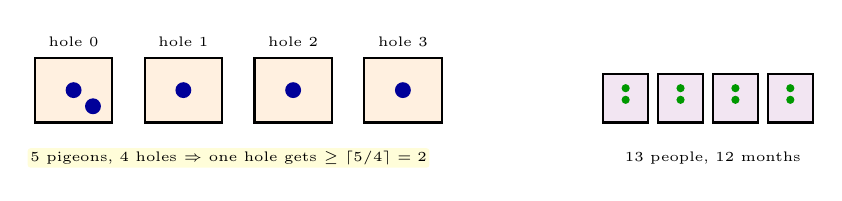
\begin{tikzpicture}[scale=0.82,every node/.style={font=\scriptsize}]
% Pigeonhole visual
\foreach \i in {0,...,3} {\draw[thick,fill=orange!12] (\i*1.7,0) rectangle++(1.2,1.0); \node[font=\tiny] at (\i*1.7+0.6,1.25) {hole \i};}
% 5 pigeons into 4 holes forces collision
\foreach \x/\y in {0.6/0.5,2.3/0.5,4.0/0.5,5.7/0.5,0.9/0.25} \fill[blue!60!black] (\x,\y) circle (3.5pt);
\node[font=\tiny,fill=yellow!15,rounded corners=1pt,inner sep=1pt] at (3.0,-0.55) {5 pigeons, 4 holes $\Rightarrow$ one hole gets $\ge\lceil5/4\rceil=2$};
% Example: among 13 people, 2 share birth month
\begin{scope}[xshift=8.8cm]
\foreach \i in {0,...,3} {\draw[thick,fill=violet!10] (\i*0.85,0) rectangle++(0.7,0.75);}
\foreach \i in {0,...,7} {\pgfmathsetmacro{\x}{mod(\i,4)*0.85+0.35} \pgfmathsetmacro{\y}{0.35+int(\i/4)*0.18} \fill[green!60!black] (\x,\y) circle (1.8pt);}
\node[font=\tiny] at (1.7,-0.55) {13 people, 12 months};
\end{scope}
\end{tikzpicture}
\caption{Pigeonhole: more items than boxes forces a collision. Generalised quantifies the overload.}
\label{fig:pigeonhole}
\end{figure}

\begin{example}
Among $13$ people, two share a birth month ($13>12$). In any $n+1$ integers, two differ by a multiple of $n$ (remainders mod $n$ are $n$ holes).
\end{example}

\begin{theorem}[Stars and bars]
Number of $k$-tuples $(x_1,\dots,x_k)$ with $x_i\ge0$ integers and $\sum x_i=n$ is $\binom{n+k-1}{k-1}$. Picture $n$ stars and $k-1$ bars.
\end{theorem}

Inclusion--exclusion extends complement: $|A\cup B|=|A|+|B|-|A\cap B|$, $|A\cup B\cup C|=\sum|A_i|-\sum|A_i\cap A_j|+|A\cap B\cap C|$.

Product counts sequential choices, sum counts alternative choices, together they build most counts.
Tree diagrams make product and sum visible: branching width multiplies, separate trees add.
Permutations count orderings, combinations count selections, the $r!$ factor is the bridge between them.
Pascal's recurrence builds binomial coefficients from smaller ones, mirroring combinatorial reasoning.
Stars and bars turns integer compositions into placements of separators among stars.
Inclusion--exclusion generalises the Venn lens correction to any number of overlapping sets.
Pigeonhole is the Dirichlet principle: more items than boxes guarantees a collision, quantified by $\lceil n/m\rceil$.
Complement counting often simplifies at least one or at least two problems dramatically.
Binomial theorem expands powers by counting how many factors contribute each variable.
Lattice path counting shows combinatorics is geometry: every path is a binary string of rights and ups.
Product counts sequential choices, sum counts alternative choices, together they build most counts.
Tree diagrams make product and sum visible: branching width multiplies, separate trees add.
Permutations count orderings, combinations count selections, the $r!$ factor is the bridge between them.
Pascal's recurrence builds binomial coefficients from smaller ones, mirroring combinatorial reasoning.
Stars and bars turns integer compositions into placements of separators among stars.
Inclusion--exclusion generalises the Venn lens correction to any number of overlapping sets.
Pigeonhole is the Dirichlet principle: more items than boxes guarantees a collision, quantified by $\lceil n/m\rceil$.
Complement counting often simplifies at least one or at least two problems dramatically.
Binomial theorem expands powers by counting how many factors contribute each variable.
Lattice path counting shows combinatorics is geometry: every path is a binary string of rights and ups.
Product counts sequential choices, sum counts alternative choices, together they build most counts.
Tree diagrams make product and sum visible: branching width multiplies, separate trees add.
Permutations count orderings, combinations count selections, the $r!$ factor is the bridge between them.
Pascal's recurrence builds binomial coefficients from smaller ones, mirroring combinatorial reasoning.
Stars and bars turns integer compositions into placements of separators among stars.
Inclusion--exclusion generalises the Venn lens correction to any number of overlapping sets.
Pigeonhole is the Dirichlet principle: more items than boxes guarantees a collision, quantified by $\lceil n/m\rceil$.
Complement counting often simplifies at least one or at least two problems dramatically.
Binomial theorem expands powers by counting how many factors contribute each variable.
Lattice path counting shows combinatorics is geometry: every path is a binary string of rights and ups.
Product counts sequential choices, sum counts alternative choices, together they build most counts.
Tree diagrams make product and sum visible: branching width multiplies, separate trees add.
Permutations count orderings, combinations count selections, the $r!$ factor is the bridge between them.
Pascal's recurrence builds binomial coefficients from smaller ones, mirroring combinatorial reasoning.
Stars and bars turns integer compositions into placements of separators among stars.
\begin{remark}[Overcounting pitfall]
Counting ordered then dividing by symmetry is powerful but error-prone: ensure each object is overcounted equally. For ``choose a pair then an extra'' counts, check if the extra could have been in the pair.
\end{remark}

\begin{example}[Committee with overlap]
Choose $3$ from $10$ then a leader among $3$: $ \binom{10}{3}\cdot3$. Alternative: choose leader first ($10$ ways) then $ \binom{9}{2}$ others: $10\binom{9}{2}$ --- same count. Two viewpoints, one answer.
\end{example}


\begin{theorem}[Binomial theorem]
$(x+y)^n=\sum_{k=0}^{n}\binom{n}{k}x^{n-k}y^k$. Combinatorial: choose $k$ factors contributing $y$.
\end{theorem}

\begin{example}[Lattice paths]
Monotone paths from $(0,0)$ to $(m,n)$ moving right/up: $\binom{m+n}{m}$ (choose which steps are right).
\end{example}

\subsection{Conditional Probability and Bayes' Theorem}
\label{sec:bayes}
Counting becomes probability on dividing by the sample size: $P(A)=|A|/|\Omega|$. \emph{Conditional} probability zooms into the $B$-world: $P(A\mid B)=|A\cap B|/|B|=P(A\cap B)/P(B)$. Flipping the condition is \emph{Bayes' theorem}: $P(H\mid E)=P(E\mid H)P(H)/P(E)$---update belief in hypothesis $H$ after seeing evidence $E$.
\begin{example}[Base-rate check]
$1\%$ of mail is spam ($P(S)=0.01$). A filter flags $95\%$ of spam but also $5\%$ of legit mail. Given a flag $F$: $P(S\mid F)=0.95\cdot0.01/(0.95\cdot0.01+0.05\cdot0.99)=0.0095/0.059\approx0.16$. Most flags are false alarms---the base rate dominates. Always expand $P(E)$ by total probability first.
\end{example}

\section{Worked Example: Two Ways to Count}
Count the number of binary strings of length $n$ with exactly $k$ ones: $\binom{n}{k}$ (choose positions for ones). Now count the same set by complement: strings with $\ge k$ ones = total $2^n$ minus strings with $<k$ ones. For $n=5,k=3$, $\binom{5}{3}=10$, and $\sum_{i=0}^{2}\binom{5}{i}=1+5+10=16$, so $\ge3$ has $32-16=16$; indeed $\binom{5}{3}+\binom{5}{4}+\binom{5}{5}=10+5+1=16$.

Stars and bars worked: distribute $10$ identical cookies to $3$ children. Put $10$ stars in a row, insert $2$ bars to split into $3$ blocks: e.g.\ $***|****|***$ means $3,4,3$. Number of placements of $2$ bars among $12$ positions $=\binom{12}{2}=66$. If each child must get $\ge1$, pre-give $1$ each, then distribute $7$ remaining: $\binom{9}{2}=36$.

% ============================================================
\section{Chapter Notes}
Combinatorics predates computers but underpins complexity counting and probability analysis of algorithms. Binomial coefficients appear in complexity bounds and generating functions (Ch.~6). The pigeonhole principle appears everywhere from hashing collisions to lower bounds.

% ============================================================
\section{Exercises}
\label{sec:ch05-exercises}
\begin{enumerate}[label=E5.\arabic*, leftmargin=*, itemsep=0.6em]
\item \textbf{Product/sum.} How many $4$-character strings with $2$ letters then $2$ digits have no repeated character? How many have at least one digit repeated? Use complement.
\item \textbf{Permutations vs combinations.} A team of $3$ from $10$ plus a leader among the $3$: count two ways and explain the factor $3$.
\item \textbf{Binomial.} Prove $\binom{n}{r}=\binom{n}{n-r}$ combinatorially and verify Pascal $\binom{5}{2}= \binom{4}{1}+\binom{4}{2}$ via counting.
\item \textbf{Pigeonhole.} Show among any $5$ points in a unit square, two are at distance $\le\sqrt2/2$ (partition into $4$ quarter-squares).
\item \textbf{Stars and bars.} Count solutions to $x_1+x_2+x_3=10$ with $x_i\ge0$; then with $x_i\ge1$ (shift $y_i=x_i-1$). Relate to $\binom{n}{r}$.
\end{enumerate}
% End of Chapter 5
